\documentclass[letter,twocolumn]{report}
\date{February 15, 2020}
\author{Nathan Louck}



%Formatting Packages
\usepackage{graphicx}
\usepackage{wrapfig}
\usepackage{anyfontsize}
\usepackage{multicol}
\usepackage{blindtext}
\usepackage{color}
\usepackage{subcaption}
\usepackage[margin=0.625in]{geometry}
\usepackage[export]{adjustbox}
\usepackage[shortlabels]{enumitem}

%For adding PDF final cover & datasheets
\usepackage{pdfpages}
\usepackage[toc,page]{appendix}

%For bibliography 
\usepackage[backend=bibtex,style=ieee]{biblatex}
\addbibresource{refs.bib}
\bibstyle{numeric}

%For URLs
\usepackage{hyperref}
\usepackage{url}
\usepackage{keyval}
\usepackage{ifthen}

% xColor - used for "listings" packagesadf
\usepackage{xcolor}
	\definecolor{dkgreen}{rgb}{0,0.6,0}
	\definecolor{gray}{rgb}{0.5,0.5,0.5}
	\definecolor{mauve}{rgb}{0.58,0,0.82}

% Listings Package for Code Block formatting
\usepackage{listings}
	% Define code block style
	\lstset{frame=tb,
		language=Python,
		aboveskip=3mm,
		belowskip=3mm,
		showstringspaces=false,
		columns=flexible,
		basicstyle={\scriptsize\ttfamily},
		numbers=none,
		numberstyle=\tiny\color{gray},
		keywordstyle=\color{blue},
		commentstyle=\color{dkgreen},
		stringstyle=\color{mauve},
		breaklines=true,
		breakatwhitespace=true,
		tabsize=3
	}

% Titlesec - for formatting section and subsection headings
\usepackage{titlesec}
	% format title, section, subsection, etc.

	\renewcommand\thesection{\Roman{section}}
	\titleclass{\section}{top}
	\titleformat{\section}{\titlerule\centering\LARGE\bfseries}{\thesection{}}{5pt}{}
	\titleformat{\subsection}{\Large\bfseries}{}{0pt}{}
	\appendicestocpagenum


% 5/4/20 from Mario
% Adding new sections:
%*% 1- Add an "Introduction" section where you describe the general idea of the project and its objective. I think your Abstract section can be renamed as an Introduction section, and you can write a more concise Abstract at the beginning. Abstract should be around 150-200 words at most.
% 2- You need to add a section on Performance Results, where you show the graphs of the gas sensor, light sensor and the measurement from the camera (or the audio measurements).
% 3- You need to add a Conclusion and a Bibliography section. References should be listed in a Bibliography section at the end of the report (and not as Footnotes). You can use in-text citation to refer to each bibliography item in the text.

% Missing parts:
% 1- There was no discussion about the motion sensor. This section should be added, in addition to the code that was used to read digital data.
% 2- You need to add the detailed computation of the gas sensor and PPM measurements (from Ashish's report).
% 3- You need to add a section including the Python codes that were used to read both analog and digital data, explaining briefly the function of each code.
% 4- Include a block diagram showing the connection among the different system components (Raspberry Pi to sensors, etc.)

% Report structure:
% 1- You need to add references for the Zigbee protocol in section IV
% 2- In page 6 (Raspberry Pi), remove the question mark before GHz
% 3- List of figures, page 15, should be moved after the table of content.

% Please try to make these changes and send me your final report by May 8th.

\begin{document}
	\large
	\begin{titlepage}
		\begin{center}
	\large
	Oswego State University of New York \\ 
	\vspace{2.5in}

	Automated Home Security [Preliminary Report v0505\_3] \\ 
	\tiny\textit{(THIS COVER WILL BE REPLACED WITH DEPARTMENT MANDATED VERSION)}\\
	\vspace{2in}
	\normalsize 
	Ashish Kharka, Jonathan Castillo, Nathan Loucks \\
	\vspace{0.5in}
	\small\textit{
		Submitted in Partial Fulfillment of the Requirement for the B.Sc. Degree, 	\\Electrical and Computer Engineering Department
		}
\end{center}
	
	\newpage
		\section{Acknowledgments}
		\begin{center}
\vspace{0.25\textheight}
\par We would like to express our gratitude to Dr. Mario Bkassiny, for his continuous support and guidance.  \\ 
\vspace{1em}
\par Our sincere thanks goes to Dennis Quill for his help and advice on parts as well as his expertise working with Raspberry Pi devices. \\ 
\vspace{1em}
\par Finally we would like to thank the ECE department as a whole for providing the resources necessary to make this research possible despite having to work remotely due to the unique circumstances of the spring 2020 semester. Without the planning and preparation made by the ECE department this project and many others would not have been possible. 
\end{center}
	\end{titlepage}
		
	\subsection{Abstract}
		% ABSTRACT
{\small\bf
	\par Abstract — Modern security systems more often than are not very consumer friendly in their business practices. Most home security companies charge a large amount of money for initial installation and some other companies require a subscription based payment method to have your home secure. With the use of a couple inexpensive electronic components one can implement a security system of their own. 
}
	\subsection{Introduction}
		\par Home security systems are becoming a staple for home owners in America. The expansion of the embedded systems market over the past few decades has made microprocessors and embedded RF communication commonplace in today's society. Most cell phones today contain several of these devices with WiFi, Bluetooth, GSM, and even satellite navigation right in your pocket. In the home, many people are using “Smart Home” devices such as voice assistants, automated thermostats and light switches. As these devices have gained a significant amount of popularity in recent years, “Smart” home security is also a rapidly growing trend. 
	\par There are a plethora of viral videos out there showing footage of criminal activity occurring right outside someone's home, without their home security system they may have never been alerted to any potential danger. 
	\par In a study released in 2010\cite{Catalano} by the U.S. Department of Justice, Bureau of Justice Statistics, an estimated 3.7 million burglaries occurred annually over preceding years. About 12\% of homes burglarized while the occupant was present resulted in the homeowner facing an offender armed with a firearm or other deadly weapon. 
	\par A security system of any complexity is a good step in the pursuit of ensuring that you and your loved ones are protected home. The autonomous nature of our system has the added advantage of operating in a stand-alone fashion, sparing the homeowner the trouble of setting an alarm or monitoring the sensors them self. 
	\par Most modern security systems have sensors that can detect carbon monoxide and motion or glass-break, and record and send live video for the user to view remotely. This provides a safer living environment for the occupants when they’re home or away, as well as peace of mind. Major security companies often require a service or subscription that a user pays periodically, as well as relatively complicated installation.  
	\par An inexpensive and easy to use home security system would let the user take control of their own home security. Making erstwhile wired sensors operate over a wireless channel would allow for the greatest ease of use for a typical consumer. 
	\par Using XBee RF modules and a Raspberry Pi, one can create their own automated home security system with the aforementioned functionalities. The XBee modules are used as communication devices that report sensor data back to a main unit, housing a system that processes the data and responds accordingly.The Raspberry Pi will serve as the main control unit to coordinate the signals coming from each sensor module, as well as transmit  or store video depending on user configuration.. The goal of this project is to create an automated home security system that is inexpensive yet delivers the user a range of  key capabilities to help protect their home and loved ones from preventable harm. 

	
	
	\subsection{Student Statement}
		As one of the final steps in the pursuit of our degrees, this project has been a long but rewarding process. The Spring 2020 semester was significantly impacted by the COVID-19 outbreak. 
\par All of us, students and staff, were required to come up contingencies on short notice to facilitate the completion of our projects. As a result we needed to find solutions not only to the problems initially proposed, but also to the new problems created by the aberrant situation. 
\par Our erstwhile well planned timeline was thrown entirely out the window. Luckily, we had been ahead of schedule prior to the transition to remote collaboration. Within a short time we had a tentative plan to bring our system to fruition. Ultimately our end product lacks some functionality that was initially proposed due to a variety of extenuating factors, beyond our control. 

	\tableofcontents
	\listoffigures

	\section{Research and Design}
		\subsection{The XBee S2C Module}
			\par For the heart of this wireless system we decided to use the XBee IEEE 802.15.4 RF modules manufactured by Digi International. These light weight, low-power modules are idea for this type of system given the desired ranges and performance characteristics we were looking for. To make a suitable home security system, the transfer of information from point A to B must be fast but reliable, and without errors or interference.
 \par IEEE 802.15.4 standard is a member of the 802.15 group of standards for wireless personal area networks (WPAN) and is used for a wide variety of applications. In our case, the implementation of this standard in the XBee modules provides an adequate range, about 200 ft (60 m) in an indoor environment, as well as an adequate data transfer speed of 250 Kbps over the 2.4 GHz RF channel.     
\par The nodes we designed around the XBee modules are battery operated and thus must have relatively low power consumption. The XBee modules themselves draw a maximum of 45 mA when transmitting, 31 mA when receiving, and less than 1 $\mu$A when in the powered down state. 
\par The XBee modules come complete with 15 I/O pins and multiple analog to digital converters. This makes them the perfect choice for data acquisition of remote sensors. 
\par XBee modules are available in a variety of form factors. We chose the XB24CAPIT form factor for our designs. Its antenna is contained within the PCB, while this may have less range than a wire antenna or U.fl add-on type of antenna, it provides excellent range for our application with minimal complexity. This model XBee is through-hole mounted, making initial designs and testing much easier that with a surface mount variety, though these occupy a smaller rectangular footprint. 
\par All of these considerations taken into account we decided that the XBee-XB24CAPIT would be the ideal communication module for the system we have designed. \\

\subsubsection{API vs Transparent Mode}
\begin{table}[h]\cite{Digi}
	\begin{tabular}[width=0.5\linewidth]{p{0.5\linewidth}p{0.5\linewidth}}
		API & Transparent \\
		\hline
			 Sends wireless data to multiple destinations. &Provides a simple interface that makes it easy to get started with XBee devices. \\
			Can set or read the configuration of remote XBee devices in the network.&what you send is exactly what other modules get, and vice versa.\\
			Can transmit data to one or multiple destinations&Works very well for two-way communication between XBee devices.
	\end{tabular}
\end{table}
		\subsection{Raspberry Pi}
			\par The Raspberry Pi 3 Model A+ is the latest product in the Raspberry Pi 3 range, weighing in at just 29 g. Like the Raspberry Pi 3 Model B+, it boasts a 64-bit quad core processor running at 1.4?GHz, dual-band 2.4?GHz and 5?GHz wireless LAN, and Bluetooth 4.2/BLE. The dual-band wireless LAN comes with modular compliance certification, allowing the board to be designed into end products with significantly reduced wireless LAN compliance testing, improving both cost and time to market. The Raspberry Pi 3 Model A+ has the same mechanical footprint as the older Raspberry Pi 1 Model A+.
	\begin{figure}[h]
		\centering
		\includegraphics[width=3in]{rasPi.png}
		\caption{Raspberry Pi 3 Model A+}
	\end{figure}
\subsubsection{Raspberry Pi Camera (Hardware and Software)}
\par The Raspberry Pi Camera v2 is the new official camera board released by the Raspberry Pi Foundation. The Raspberry Pi Camera Module v2 is a high quality 8 megapixel Sony IMX219 imagesensor custom designed add-on board for Raspberry Pi, featuring a fixed focus lens. It's capable of 3280 x 2464 pixel static images, and also supports 1080p30, 720p60 and 640x480p90 video. It attaches to Pi by way of one of the small sockets on the board upper surface and uses the dedicated CSi interface, designed especially for interfacing to cameras.
\begin{figure}[h]
	\centering
	\includegraphics[width=2in]{picam.jpg}
	\caption{PiCamera Python Module}
\end{figure}
\par This package provides a pure Python interface to the Raspberry Pi camera module for Python 2.7 (or above) or Python 3.2 (or above). It can configure resolution and give different dimensions to the video or picture files. It can also take photos under varying conditions if given the right parameters for a camera to take a good picture under different conditions such as lighting conditions. 
The code for the camera is as follows
\begin{figure}[h]
	\includegraphics[width=2.3in]{camcode1.jpg}\\
	\includegraphics[width=0.4\textwidth]{camcode2.jpg}
\end{figure}

\subsubsection{PiCamera difficulties}
\par Camera Component sends a camera control callback error and does not take and save pictures anymore. The OS of the raspberry pi has been reset and redownloaded to the raspberry pi. There is a visible trigger to the camera activating when using the Pi NOIR camera board. There is a red light on the board of the camera that signifies when it is turned on or activated. The camera when activated through the command window will sometimes create the file but have no data inside of it. Upon receiving this error it seems to slow down the raspberry pi board significantly that it requires a restart. The raspberry pi has been test with three different camera modules and all of them give back the same callback control error.  Raspberry Pi has configuration settings to activate and recognize when a camera is connected, however the issues may seem to arise with a faulty port on the raspberry pi itself.
\begin{figure}[h]
	\begin{lstlisting}
	mmal: Received unexpected camera control callback event, 0x4f525245
	\end{lstlisting}
	\label{fig:camErr}
	\caption{Error from camera module}
\end{figure}
\par When attempting to switch to audio recording instead of using the camera the only devices available were 3.5mm jack from a headset with built in microphone. The assumption was to connect to the audio jack output of the raspberry pi, and record and listen through the headset itself. However, this is impossible due to the specifications of the raspberry pi the audio jack is meant for output only. The only way to record audio was using a 
%%%% REMOVED DETAILED LIST OF RASBERRY PI FEATURES	
%	\begin{itemize}
%		\item Processor 
%		\begin{itemize}
%			\item Broadcom BCM2837B0, Cortex-A53
%			\item 64-bit SoC @ 1.4 GHz
%		\end{itemize}
%		\item Memory
%		\begin{itemize}
%			\item 512MB LPDDR2 SDRAM
%		\end{itemize}
%		\item Connectivity
%		\begin{itemize}
%			\item 2.4 GHz and 5 GHz IEEE 802.11.b/g/n/ac wireless LAN
%			\item Bluetooth 4.2/BLE
%		\end{itemize}
%		\item Data and I/O interfacing
%		\begin{itemize}
%			\item Extended 40-pin GPIO header
%		\end{itemize}
%		\item Video and Sound
%		\begin{itemize}
%			\item 1x HDMI
%			\item MIPI DSI display port
%			\item MIPI CSI camera port
%			\item 4 pole stereo output and composite video port
%		\end{itemize}
%		\item Multimedia 
%		\begin{itemize}
%			\item H.264, MPEG-4 decode (1080p30)
%			\item H.264 encode (1080p30)
%			\item OpenGL ES 1.1, 2.0 graphics
%		\end{itemize}
%		\item SD card Support
%		\begin{itemize}
%			\item Micro SD format for loading operating system and data storage
%		\end{itemize}
%		\item Input Power Specifications
%		\begin{itemize}
%			\item 5 V/2.5 A DC via micro USB connector
%			\item 5 V DC via GPIO header
%		\end{itemize}
%	\end{itemize}
		\subsection{Python, Primary Programming Language}
			\input{python.tex}
		\subsection{Supplying Power}
			\par The next consideration to be made was supplying power. In the pursuit of making out devices truly wireless, we were determined to have all the end-point devices be completely battery operated. Though the XBee RF modules themselves use minimal power even while transmitting, an efficient power supply would be necessary for prolonged operation. 
	\begin{figure}[h]
		\centering
		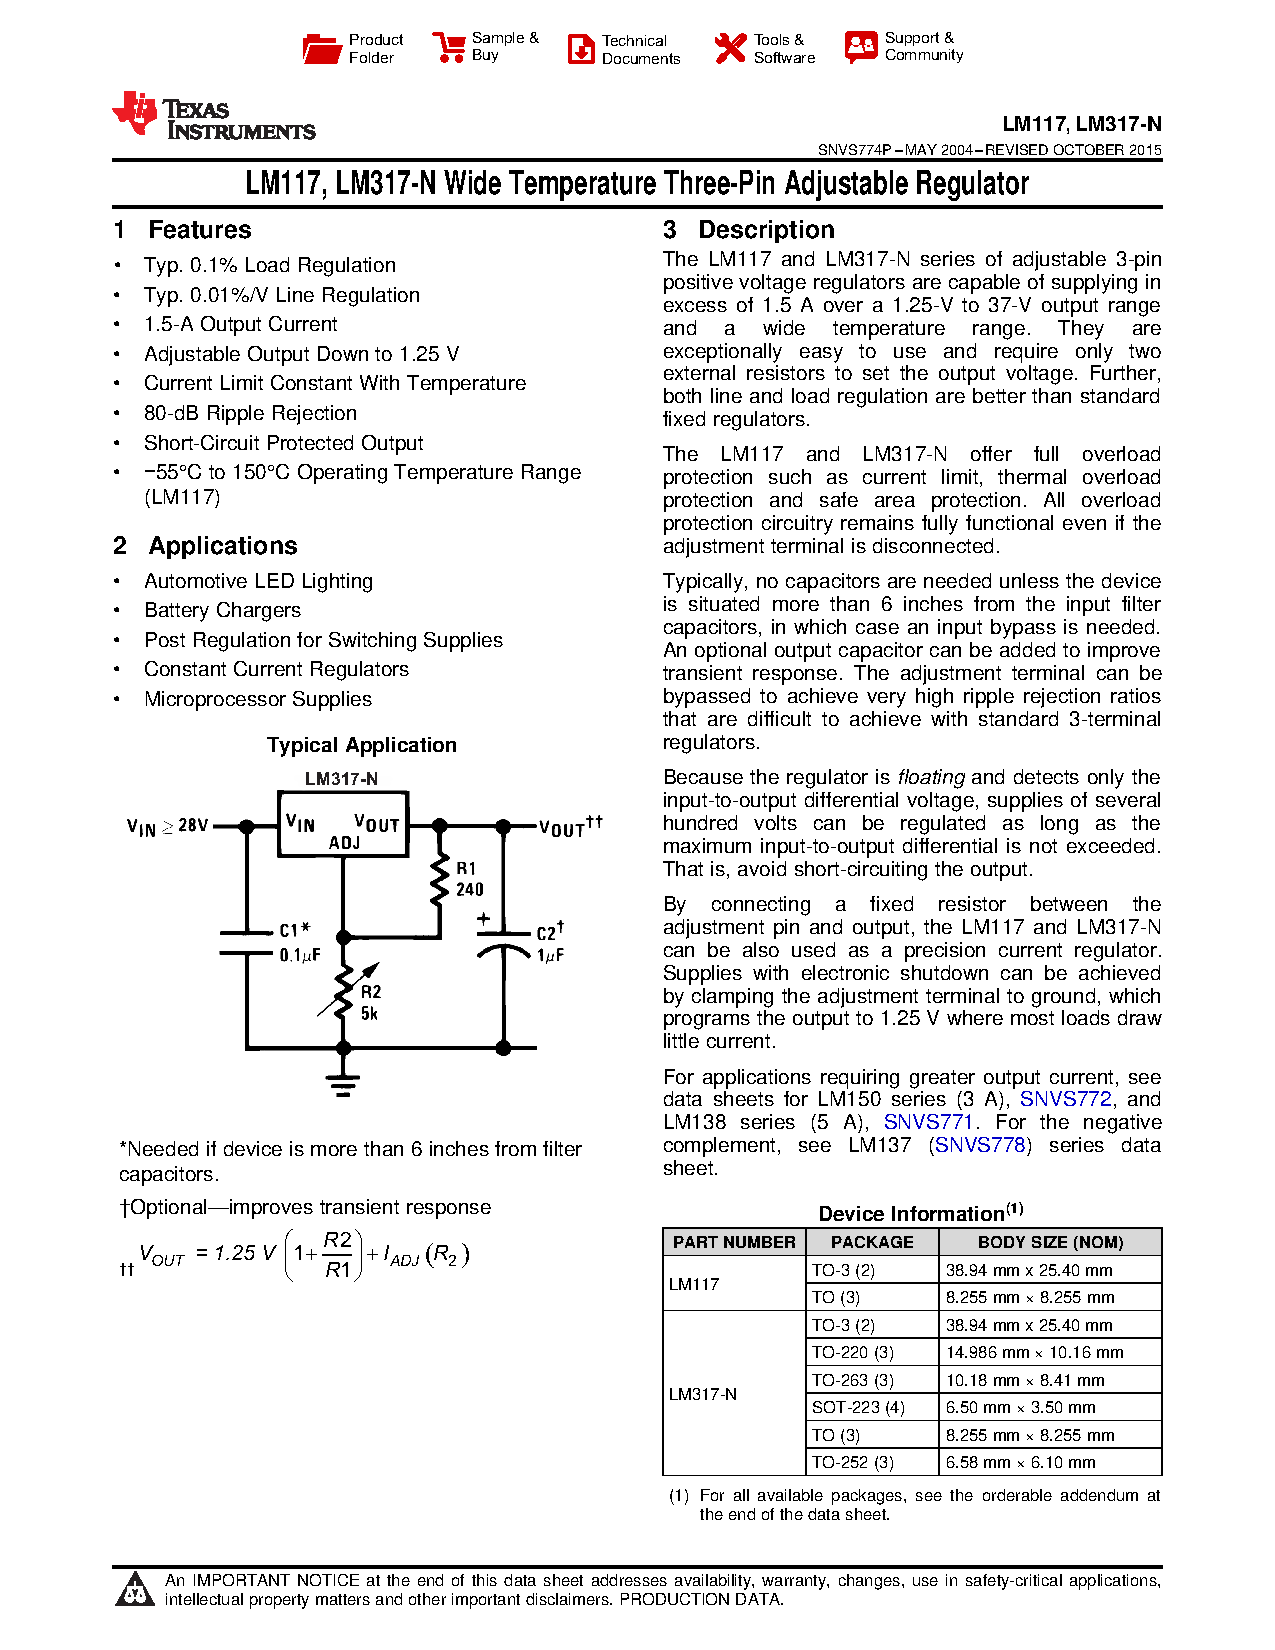
\includegraphics[width=2in]{lm317.jpg}
		\caption{\small LM317 Linear Regulator (TH)}
	\end{figure}
	\paragraph{\normalsize LM317 Linear Voltage Regulator \hspace{1.5em}} 
	The LM317 is an IC designed to maintain a constant voltage level. Voltage regulators usually have an input voltage range, but for the LM317 voltage regulator, the range is not specified because it has no ground connection. It has an output voltage range from 1.2 V to 37 V at 1.5 A. Since it is a linear regulator, the output voltage is always lower than input. The LM317 is used in our project to power the XBee modules which require a supply voltage between 2.1 V and 3.6 V. We designed a circuit incorporating the LM317 to output 3.3 V, which is ideal to power our devices. 
	\begin{figure}[h]
		\centering
		\includegraphics[width=3in]{33vsource.jpg}
		\caption{Complete power supply circuit.}
		\label{3v_circuit}
	\end{figure}
	\par As in figure \ref{3v_circuit}, the values we know are V\textsubscript{o} = 1.2 V, V\textsubscript{out} = 3.3 V and setting R1 = 330 $\Omega$.  The value of Iadj is very small hence it can have considered negligible. The value of R2 came to 550 $\Omega$. We then added the C1 = 100 $\mu$F, C2 = 0.1 $\mu$F and C3 = 10 $\mu$F for the improvement of transient response of a system to change from steady state. 
	
	\paragraph{\normalsize LM7805 5V Voltage Regulator}
	To power our devices that require a 5 volt source such as the MQ-6 LP gas sensor, we chose to design a circuit around the LM7805 voltage regulator. This regulator has an input range of 5 to 18 volts, ideal for out 6 volt battery packs, and produces a constant 5 volt output. 


	
	\subsection{Environment Monitoring Hardware}
		% sensingHardware.tex
\subsection{MQ6 Liquid Petroleum Gas Sensor}
\par The MQ-6 gas sensor is a highly sensitive sensor designed to detect different atmospheric gases, such as propane, butane and other LPG (Liquid Petroleum Gas), also response to natural gas. It can also detect different some other combustible gases, notably methane. The sensor's conductivity changes proportional to the ambient gas concentration. The relatively low cost and wide range of detection make it an excellent choice for our system. The MQ-6 sensor operates at 5-volts.
\begin{figure}[h!]
	\centering
	\begin{subfigure}[t]{0.45\textwidth}
		\centering
		\includegraphics[height = 2in]{mq6.png}
		\caption{MQ6 Liquid Petroleum Gas Sensor Package}
	\end{subfigure}
	\begin{subfigure}[t]{0.45\textwidth}
		\centering
		\includegraphics[height = 1.5in]{mq6diag.png}
		\caption{MQ6 Liquid Petroleum Gas Sensor Diagram}
	\end{subfigure}
	\caption{MQ6 Gas Sensor}
\end{figure}
\subsection{Parallax Passive Infra-red Motion Sensor}\cite{Webster}
\par To trigger subsequent elements of the proposed system we needed a motion detecting sensor. An infra red motion sensor works through applying the concept of pyroelectricity, a characteristic of materials that will generate a potential difference when heated. In this case the heat source is reflected infra red light. When there is no movement, current through a resistor in series with the pyroelectric material's electrodes will be constant. When movement occurs in the field of view of the infra red source, the amount of reflected light will change causing a change in the pyroelectric voltage. This change in voltage causes the current through the circuit to change, this is measured triggers the output accordingly.\cite{Webster}
\begin{figure}[h]
	\centering
	\includegraphics{pirDevice.jpg}
	\caption{PIR Motion Sensing Module}
\end{figure}
\newpage
\par In our case, we desire a sensor such that negligible movement will be ignored. If this input was to trigger a camera, picking up a very small object's movement or similar "false alarms" would result in an over abundance of images taking up memory on the users pc or the system itself. Moreover if this device triggered an alarm, false alarms would be unacceptable in most cases. Most infra-red motion sensors on the market today are all-in-one units that take this into consideration by only raising a digital output high when a sufficiently large current change in the pyroelectric circuit is measured by the sensor module. 
\par For our system we chose to use a Parallax passive infra-red \textit{(PIR)} motion sensor. This PIR motion sensor operates from 3 volts to 6 volts meaning it can utilize the same power source as the XBee modules. The XBee will read the digital signal generated by the PIR sensor to trigger the rest of the system remotely.

		% CONTAINS:
			%\subsection{MQ6 Liquid Petroleum Gas Sensor}
			%\subsection{Parallax PIR Motion Sensor}
	
	\subsection{Hardware Testing}
		\subsubsection{Testing the MQ6 gas sensor}
\par Next, we wanted to test this sensor independently. To do this we first started off with reading the data-sheet to find out the appropriate voltage input and pin layout. We found out that it operates at 5 volts with a minimum of 0 volts. We supplied 5 volts from the power supply to our breadboard and we used an LED to our output pin to see if it detects any gas. 
\begin{figure}[h!]
	\centering
	\begin{subfigure}[t]{0.45\textwidth}
		\centering
		\includegraphics[height=1.5in]{mq6Test.png}
		\caption{LED on via pin 18}
	\end{subfigure}
	\begin{subfigure}[t]{0.45\textwidth}
		\centering
		\includegraphics[height=1.5in]{mq6TestOn.png}
		\caption{LED off via pin 18}
	\end{subfigure}
	\caption{Simple LED activation over 802.15.4 (2)}
\end{figure}
\par Properly connected, the gas sensor produced quantifiable results. Using a common butane lighter, we tested the sensors ability to detect ambient gases. The LED was able to indicate the presence of LPG, thus we now know our gas sensing components are functional.
\par Since the XBee modules analog to digital converter requires an input in the range of 1.2 volts, we must reduce the 5 volt output of the gas sensor down to this level to be quantified and processed. To do this a simple voltage divider was designed (1). With voltages constant and one resistor value constant we only need to solve for one unknown (2).
\begin{equation}
V\textsubscript{out}=\frac{R1}{R1+R2}*V\textsubscript{in}
\end{equation}
Solving for R1: \\
\begin{equation}
1.2 = \frac{5100}{R1+5100}*5
\end{equation}
\[R1 = 16150 \Omega\]

% Testing the PIR Motion sensor
\subsubsection{Testing the PIR Motion Sensor}
\par The Parallax sensor allows us to choose between two set trip duration options, either an approximate time of 2 seconds or 5 seconds. This means that when the sensor is triggered it will hold its output high for the selected option. This setting is changed with the manual moving of a jumper that connects a center pin with a second pin either on its left or right. In essence this is a crude switch. To yield as flexible a system as possible, a small DIP switch has been designed to toggle this setting. This allows the user to decide between a "Shorter" or "Longer" setting depending on which is best suited to their operating environment. This would be set to the "Shorter" option by default. 
\par In initial testing of the sensor, the output received at the XBee itself was subject to some instability. This was solved by adding an RC filter between the digital input of the XBee and the output of the sensor module. This eliminated a DC component that would sometimes be present in the signal. 

 


\subsubsection{Testing Raspberry Pi \& Camera}
\paragraph{Camera difficulties} Camera Component sends a camera control callback error and does not take and save pictures anymore. The OS of the raspberry pi has been reset and redownloaded to the raspberry pi. There is a visible trigger to the camera activating when using the Pi NOIR camera board. There is a red light on the board of the camera that signifies when it is turned on or activated. The camera when activated through the command window will sometimes create the file but have no data inside of it. Upon receiving this error it seems to slow down the raspberry pi board significantly that it requires a restart. The raspberry pi has been test with three different camera modules and all of them give back the same callback control error.  Raspberry Pi has configuration settings to activate and recognize when a camera is connected, however the issues may seem to arise with a faulty port on the raspberry pi itself.
\begin{figure}[h]
	\begin{lstlisting}
	mmal: Received unexpected camera control callback event, 0x4f525245
	\end{lstlisting}
	\label{fig:camErr}
	\caption{Error from camera module}
\end{figure}
\par When attempting to switch to audio recording instead of using the camera the only devices available were 3.5mm jack from a headset with built in microphone. The assumption was to connect to the audio jack output of the raspberry pi, and record and listen through the headset itself. However, this is impossible due to the specifications of the raspberry pi the audio jack is meant for output only. The only way to record audio was using a 

	\subsection{Physical Construction of End-point Devices}
	\par The modules themselves will be constructed on 6x8 cm perf-board and will be contained in a housing. Each module will contain all circuitry necessary including power, data acquisition and transmission. 
	\begin{figure}[h!]
		\centering
		\begin{subfigure}[t]{0.45\textwidth}
			\centering
			\includegraphics[height=1.5in]{module_gas.jpg}
			\caption{Gas Module}
		\end{subfigure}
		\begin{subfigure}[t]{0.45\textwidth}
			\centering
			\includegraphics[height=1.5in]{module_motion.jpg}
			\caption{Motion Module}
		\end{subfigure}
		\caption{Internals of Gas (a), and Motion (b) sensing units}
	\end{figure}
	\par The gas sensor module requires two power supplies, one 3.3 volts to power the XBee itself and 5 volts to operate the Tin Dioxide (SnO2) gas sensor. \\
	\par Our system consists of 4 separate modules:
	\begin{itemize}
		\item Coordinator Module - Connects directly to the PC, connects to user interface and controls messages between subsequent end point modules. 
		\item LP Gas Module - A liquid petroleum gas sensor to detect gas leaks in the home. Can detect a wide range of flammable gasses commonly found a typical home.
		\item Motion Sensing Module - The motion sensing module will detect movement and trigger a system response to suit. The Motion module is stand alone to allow the as much freedom of placement as possible.
		\item Door Camera/Lock Module - This module, when directed to do so, can take an image of the area as well as lock the door automatically. This is the most complicated module in the system and includes a Raspberry Pi to transfer frames over the local area network.
	\end{itemize}

	
	\subsection{Creating the Wireless Network between the Coordinator and Router modules}
	\par We wanted to create a wireless network between the coordinator and router modules this time. Firstly, we started off with soldering our XBee Explorer to connect our router modules on top of them. The reason we chose Xbee Explorer was because it will allow us to solder the input power voltage and the output pins that will be connected to the sensors. We used the application XCTU to help us set up each Xbee as a coordinator or router modules. We first set our coordinator in API mode that will allow us to communicate directly with the sensors via router modules. At the same time, we set the other three router modules to be in a AT or Transparent mode. This will allow sensors to send data directly to the coordinator. We also made sure all the XBee modules used the same Channel and Personal area network (PAN) ID. 
	\begin{figure}[h]
		\centering
		\includegraphics[width = 0.3\textwidth]{xbeeMiniExplorer.png}
		\caption{Small XBee interface to be used in each module}
	\end{figure}
	\subsection{Controlling the Router XBee with XCTU Remote AT Command}
	\par We decided to test our router XBee remotely by sending some AT Commands. We used the XCTU application to first create the Remote AT Command to turn on and off pin 18 of the router XBee. To see if we receive any output, we put an LED to see if the pin was turned on or not. In the figure below you can see the LED turning on and off via Pin 18 of the XBee device. The pictures help visualize what the pin is doing corresponding to the LED.
	\begin{figure}[h!]
		\centering
		\begin{subfigure}[t]{0.22\textwidth}
			\centering
			\includegraphics[width=\textwidth]{xbeeXctu1.png}
			\caption{Turn On Pin 18}
		\end{subfigure}
		\begin{subfigure}[t]{0.22\textwidth}
			\centering
			\includegraphics[width=\textwidth]{xbeeXctu1.png}
			\caption{Turn Off Pin 18}
		\end{subfigure}
		\caption{Simple LED activation over 802.15.4}
	\end{figure}
	\begin{figure}[h!]
		\centering
		\begin{subfigure}[t]{0.45\textwidth}
			\centering
			\includegraphics[height=1.5in]{ledRemoteTest.png}
			\caption{LED on via pin 18}
		\end{subfigure}
		\begin{subfigure}[t]{0.45\textwidth}
			\centering
			\includegraphics[height=1.5in]{ledRemoteTestOFF.png}
			\caption{LED off via pin 18}
		\end{subfigure}
		\caption{Simple LED activation over 802.15.4 (2)}
	\end{figure}
	\newpage
	\subsection{Controlling XBee module using Python}
	\par Since we now know that remote router XBee can be controlled by the coordinator XBee wirelessly, we decided to use python program for the same task. First, we connected our coordinator Xbee module to the computer and set it to API mode. Then we powered up the router module and now we know that it has been connected in a wireless mesh network. We used the XCTU application to generate the same Remote AT Command frame to control the pin 18 of the router module. Then opened the python program to start writing our program in a new script file. API frame generated to Turn on \& Off pin 18: 
	\begin{figure}[h!]
		\centering
		\begin{subfigure}[t]{0.22\textwidth}
			\centering
			\includegraphics[width=\textwidth]{xctuFrames1.png}
			\caption{Turn On Pin 18}
		\end{subfigure}
		\begin{subfigure}[t]{0.22\textwidth}
			\centering
			\includegraphics[width=\textwidth]{xctuFrames2.png}
			\caption{Turn Off Pin 18}
		\end{subfigure}
		\caption{API Frames created in XCTU}
	\end{figure} 
	\begin{lstlisting}
	#Configure AD2 and DIO2 to control pin-18
	
	import serial
	import binascii
	import time
	
	ser = serial.Serial(COM3)
	ser.baudrate = 9600
	
	#XCTU API Frame remote AT command used to control pin-18
	#Power ON
	turnOn = "7E 00 01 17 01 00 13 A2 00 41 82 D2 22 FF FE 02 44 32 05 01"
	#Power OFF
	turnOff = "7E 00 01 17 01 00 13 A2 00 41 82 D2 22 FF FE 02 44 32 04 02"
	
	#Use binascii to convert hex instruction to binary
	messageOn = "".join(turnOn.split()) 
	on = binascii.unhexlify(messageOn)
	
	messageOff = "".join(turnOff.split())
	off = binascii.unhexlify(messageOff)
	
	#Test write commands, flash led at 5 sec intervals
	count = 0
	while (count < 10)
		ser.write(on)
		time.sleep(5)
		ser.write(off)
		count = count + 1
	\end{lstlisting}
	
	\printbibliography		

	\begin{appendices}
		\begin{center}
			\textbf{\Huge Appendix A\label{mq6:MDS} \vfill MQ-6 LPG Sensor Data-sheet}
			
		\end{center}

		\includepdf{MQ6.pdf}
		
		\begin{center}
			\textbf{\vspace{0.35\textheight}\Huge Appendix B\label{PIR:MDS} \\Parallax PIR Motion Sensor Data-sheet}
			\newpage
		\end{center}
		\includepdf{PIRMDS.pdf}

		\begin{center}
			\textbf{\vspace{0.35\textheight}\Huge Appendix C\label{refs} \\Included Reference}
			\newpage
		\end{center}
	\end{appendices}	
\end{document}
